
%%%%%%%%%%%%%%%%%%%%%%%%%%%%%%%%%%%%%%%%%%%%%%%%%%%%%%%%%%%%%%%%%%%%%%%%%%%%%
\chapt[chap:teamware]{GATE Teamware: A Web-based Collaborative Corpus Annotation Tool}
\markboth{GATE Teamware: Web-based Annotation Tool}{GATE Teamware: Web-based Annotation Tool}
%%%%%%%%%%%%%%%%%%%%%%%%%%%%%%%%%%%%%%%%%%%%%%%%%%%%%%%%%%%%%%%%%%%%%%%%%%%%%
\nnormalsize

\def\teamware{Teamware}

%%%%%%%%%%%%%%%%%%%%%%%%%%%%%%%%%%%%%%%
%\sect[sec:family:teamware]{GATE Teamware}

Current tools demonstrate that text annotation projects can be approached successfully in a collaborative fashion. However, we believe that this can be improved further by providing a unified environment that provides a multi-role methodological framework to support the different phases and actors in the annotation process. The multi-role support is particularly important, as it enables the most efficient use of the skills of the different people and lowers overall annotation costs through having simple and efficient annotation web-based UIs for non-specialist annotators. In this paper we present \teamware, a novel web-based collaborative annotation 
environment which enables users to carry out complex corpus annotation projects, 
involving less skilled, cheaper annotators working remotely from within their web browsers. 
It has been evaluated by us through the creation of several gold standard corpora, as well as through external evaluation in commercial annotation projects. 

For technical and user interface details not covered in this chapter, please refer to the 
\htlink{http://gate.ac.uk/teamware/}{Teamware User Guide}.

GATE Teamware is open-source software, released under the GNU Affero General
Public Licence version 3.  Commercial licences are available from the
University of Sheffield.  The source code is available from the subversion
repository at

{\tt https://gate.svn.sourceforge.net/svnroot/gate/teamware/trunk}

\section{Introduction}

For the past ten years, NLP development frameworks such as OpenNLP, GATE, and UIMA have been providing tool support and facilitating NLP researchers with the task of implementing new algorithms, sharing, and reusing them.  At the same time, Information Extraction (IE) research and computational linguistics in general has been driven forward by the growing volume of annotated corpora, produced by research projects and through evaluation initiatives such as MUC \cite{Marsh98}, ACE\footnote{http://www.ldc.upenn.edu/Projects/ACE/}, DUC \cite{DUC2001}, and CoNLL shared tasks. Some of the NLP frameworks (e.g., AGTK \cite{Maeda04}, GATE \cite{Cun02b}) even provide text annotation user interfaces. However, much more is needed in order to produce high quality annotated corpora: a stringent methodology, annotation guidelines, inter-annotator agreement measures, and in some cases, annotation adjudication (or data curation) to reconcile differences between annotators. 

Current tools demonstrate that annotation projects can be approached in a collaborative fashion successfully. 
However, we believe that this can be improved further by providing a unified environment that provides a multi-role methodological framework to support the different phases and actors in the annotation process. The multi-role support is particularly important, as it enables the most efficient use of the skills of the different people and lowers overall annotation costs through having simple and efficient annotation web-based UIs for non-specialist annotators. This also enables role-based security, project management and performance measurement of annotators, which are all particularly important in corporate environments.

This chapter presents \teamware, a web-based software suite and a methodology for the implementation and support of complex annotation projects. In addition to its research uses, it has also been tested as a framework for cost-effective commercial annotation services, supplied either as in-house units or as outsourced specialist activities. 

In comparison to previous work \teamware\ is a novel general purpose, web-based annotation framework, which:
\begin{itemize}
  \item structures the roles of the different actors involved in large-scale corpus annotation (e.g., annotators, editors, managers) and supports their interactions in an unified environment;
  \item provides a set of general purpose text annotation tools, tailored to the different user roles, e.g., a curator management tool with inter-annotator agreement metrics and adjudication facilities and a web-based document tool for in-experienced annotators;
 \item supports complex annotation workflows and provides a management console with business process statistics, such as time spent per document by each of its annotators, percentage of completed documents, etc;
  \item offers methodological support, to complement the diverse technological tool support.
\end{itemize}

\section{Requirements for Multi-Role Collaborative Annotation Environments}\label{sect:requirements}

As discussed above, collaborative corpus annotation is a complex process, which involves different kinds of actors (e.g., annotators, editors, managers) and also requires a diverse range of pre-processing, a user interface, and evaluation tools. Here we structure all these into a coherent set of key requirements, which arise from our goal to provide cost-effective corpus annotation. 

Firstly, due to the multiple actors involved and their complex interactions, a collaborative environment needs to {\bf support these different roles} through user groups, access privileges, and corresponding user interfaces. Secondly, since many annotation projects manipulate hundreds of documents, there needs to be a {\bf remote, efficient data storage}. Thirdly, significant cost savings can be achieved through pre-annotating corpora automatically, which in turns requires support for {\bf automatic annotation services} and their flexible configuration. Last, but not least, a {\bf flexible workflow engine} is required to capture the complex requirements and interactions. 

Next we discuss the four high-level requirements in finer-grained details.      

\subsection{Typical Division of Labour}\label{sect:multi-role-support}

Due to annotation projects having different sizes and complexity, in some cases the same person might perform more than one role or new roles might be needed. For example, in small projects it is common that the person who defines and manages the project is also the one who carries out quality assurance and adjudication. Nevertheless these are two distinct roles (manager vs editor), involving different tasks and requiring different tool support.   

{\bf Annotators} are given a set of annotation guidelines and often work on the same document independently. This is needed in order to get more reliable results and/or measure how well humans perform the annotation task (see more on Inter-Annotator Agreement (IAA) below). Consequently, manual annotation is a slow and error-prone task, which makes overall corpus production very expensive. In order to allow the involvement of less-specialised annotators, the manual annotation user interface needs to be simple to learn and use.  In addition, there needs to be an automatic training mode for annotators where their performance is compared against a known gold standard and all mistakes are identified and explained to the annotator, until they have mastered the guidelines. 

Since the annotators and the corpus editors are most likely working at different locations, there needs to be a communication channel between them, e.g., instant messaging. If an editor/manager is not available, an annotator should also be able to mark an annotation as requiring discussion and then all such annotations should be shown automatically in the editor console. In addition, the annotation environment needs to restrict annotators to working on a maximum of \emph{n} documents (given as a number or percentage), in order to prevent an over-zealous annotator from taking over a project and introducing individual bias. Annotators also need to be able to save their work and, if they close the annotation tool, the same document must be presented to them for completion the next time they log in.  

From the user interface perspective, there needs to be support for annotating document-level metadata (e.g., language identification), word-level annotations (e.g., named entities, POS tags), and relations and trees (e.g., co-reference, syntax trees). Ideally, the interface should offer some generic components for all these, which can be customised with the project-specific tags and values via an XML schema or other similar declarative mechanism. The UI also needs to be extensible, so specialised UIs can easily be plugged in, if required. 

{\bf Editors} or curators are responsible for measuring Inter-Annotator Agreement (IAA), annotation adjudication, gold-standard production, and annotator training. They also need to communicate with annotators when questions arise. Therefore, they need to have wider privileges in the system. In addition to the standard annotation interfaces, they need to have access to the actual corpus and its documents and run IAA metrics. They also need a specialised adjudication interface which helps them identify and reconcile differences in multiply annotated documents. For some annotation projects, they also need to be able to send a problematic document back for re-annotation. 

{\bf Project managers} are typically in charge of defining new corpus annotation projects and their workflows, monitoring their progress, and dealing with performance issues. Depending on project specifics, they may work together with the curators and define the annotation guidelines, the associated schemas (or set of tags), and prepare and upload the corpus to be annotated. They also make methodological choices: whether to have multiple annotators per document; how many; which automatic NLP services need to be used to pre-process the data; and what is the overall workflow of annotation, quality assurance, adjudication, and corpus delivery.  

Managers need a project monitoring tool where they can see: 
\begin{itemize}
\item Whether a corpus is currently assigned to a project or, what annotation projects have been run on the corpus with links to these projects or their archive reports (if no longer active). Also links to the the annotation schemas for all annotation types currently in the corpus. 
\item Project completion status (e.g., 80\% manually annotated, 20\% adjudicated).
\item Annotator statistics within and across projects: which annotator worked on each of the documents, what schemas they used, how long they took, and what was their IAA (if measured).   
\item The ability to lock a corpus from further editing, either during or after a project.
\item Ability to archive project reports, so  projects can be deleted from the active list. Archives should preserve information on what was done and by whom, how long it took, etc.  
\end{itemize}


\subsection{Remote, Scalable Data Storage}\label{sec:remote-data-store}

Given the multiple user roles and the fact that several annotation projects may need to be running at the same time, possibly involving different, remotely located teams, the data storage layer needs to scale to accommodate large, distributed corpora and have the necessary security in place through authentication and fine-grained user/group access control. Data security is paramount and needs to be enforced as data is being sent over the web to the remote annotators. Support for diverse document input and output formats is also necessary, especially stand-off ones when it is not possible to modify the original content. Since multiple users can be working concurrently on the same document, there needs to be an appropriate locking mechanism to support that. The data storage layer also needs to provide facilities for storing annotation guidelines, annotation schemas, and, if applicable, ontologies. Last, but not least, a corpus search functionality is often required, at least one based on traditional keyword-based search, but ideally also including document metadata and linguistic annotations. 

\subsection{Automatic annotation services}

Automatic annotation services can reduce significantly annotation costs (e.g., annotation of named entities), but unfortunately they also tend to be domain or application specific. Also, several might be needed in order to bootstrap all types that need to be annotated, e.g., named entities, co-reference, and relation annotation modules. Therefore, the architecture needs to be open so that new services can be added easily. Such services can encapsulate different IE modules  and take as input one or more documents (or an entire corpus). The automatic services also need to be scalable, in order to minimise their impact on the overall project completion time. The project manager should also be able to choose services based on their accuracy on a given corpus. 

Machine Learning (ML) IE modules can be regarded as a specific kind of automatic service.  A mixed initiative system \cite{Day97} can be set up by the project manager and used to facilitate manual annotation behind the scenes. This means that once a document has been annotated manually, it will be sent to train the ML service which internally generates an ML model. This model will then be applied by the service on any new document, so that this document will be partially pre-annotated. The human annotator then only needs to validate or correct the annotations provided by the ML system, which makes the annotation task significantly faster \cite{Day97}.

\subsection{Workflow Support}\label{sect:workflow-reqs}

In order to have an open, flexible model of corpus annotation processes, we need a powerful workflow engine which supports asynchronous execution and arbitrary mix of automatic and manual steps. For example, manual annotation and adjudication tasks are asynchronous.  Resilience to failures is essential and workflows need to save intermediary results from time to time, especially after operations that are very expensive to re-run (e.g. manual annotation, adjudication). The workflow engine also needs to have status persistence, action logging, and  activity monitoring, which is the basis for the project monitoring tools.

In a workflow it should be possible for more than one annotator to work on the same document at the same time, however, during adjudication by editors, all affected annotations need to be locked to prevent concurrent modifications. For separation of concerns, it is also often useful if the same corpus can have more than one active project. Similarly, the same annotator needs to be able to work on several annotation projects. 

\begin{figure}[tbh!]
\begin{center}
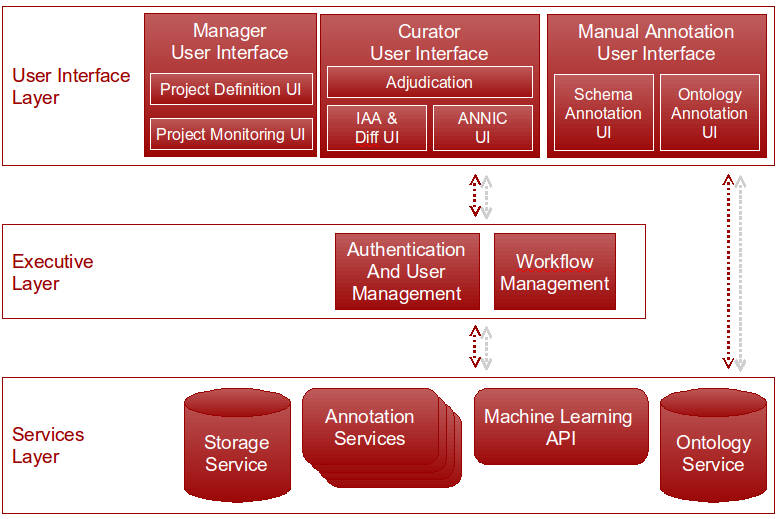
\includegraphics[scale=0.4]{teamware-arch-anon.png}
%\vspace{-4.0ex}
\caption{\teamware\ Architecture Diagram} \label{fig:architecture}
\end{center}
\end{figure}
%\vspace{-5.0ex}

\section{\teamware: Architecture, Implementation, and Examples}\label{sect:teamware}

\teamware\ is a web-based collaborative annotation and curation environment, which allows unskilled annotators to be trained and then used to lower the cost of corpus annotation projects. Further cost reductions are achieved by bootstrapping with relevant automatic annotation services, where these exist, and/or through mixed initiative learning methods. It has a service-based architecture which is parallel, distributed, and also scalable (via service replication) (see Figure~\ref{fig:architecture}). 

As shown in Figure~\ref{fig:architecture}, the Teamware architecture consists of SOAP web services for data storage, a set of
web-based user interfaces (UI Layer), and an executive layer in the middle where the workflows of the specific annotation projects are defined. The UI Layer is connected with the Executive Layer for exchanging command and control messages (such as requesting the ID for document that needs to be annotated next), and also it connects directly to the services layer for data-intensive communication (such as downloading the actual document data, and uploading back the annotations produced). 
% This is a duplicate and causes a multiply defined label error
% \begin{figure*}[tb!]
% \begin{center}
% 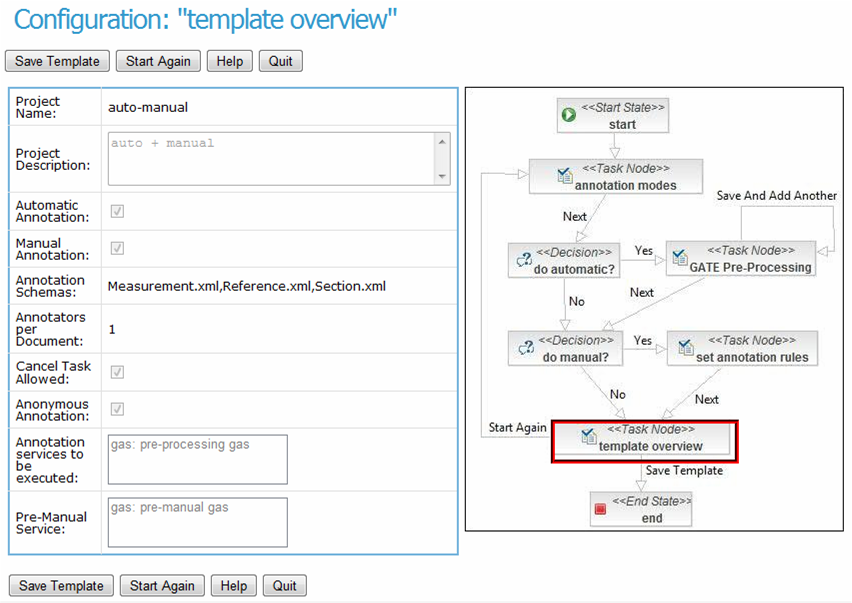
\includegraphics[scale=0.7]{treamware-workflow-example.png}
% \caption{Dynamic Workflow Configuration: Example} \label{fig:workflowExample}
% \end{center}
% \end{figure*}

\subsection{Data Storage Service}

The storage service provides a distributed data store for corpora, documents, and annotation schemas. Input documents can be in all major formats (e.g. plain text, XML, HTML, PDF), based on GATE's comprehensive support. In all cases, when a document is
created/imported in \teamware, the format is analysed and converted into GATE's single unified, graph-based model of {\em annotation}. Then this internal annotation format is used for data exchange between the service layer, the executive layer and the UI layer. Different processes within \teamware\ can add and remove annotation data within the same document concurrently, as long as two processes do not attempt to manipulate the same subset of the data at the same time.  A locking mechanism is used to ensure this and prevent data corruption.  The main export format for annotations is currently stand-off XML, including XCES \cite{Ide00a}.  Document text is represented internally using Unicode and data exchange uses the UTF-8 character encoding, so \teamware\ supports documents written in any natural language supported by the Unicode standard (and the Java platform).

\begin{figure*}[htb]
\begin{center}
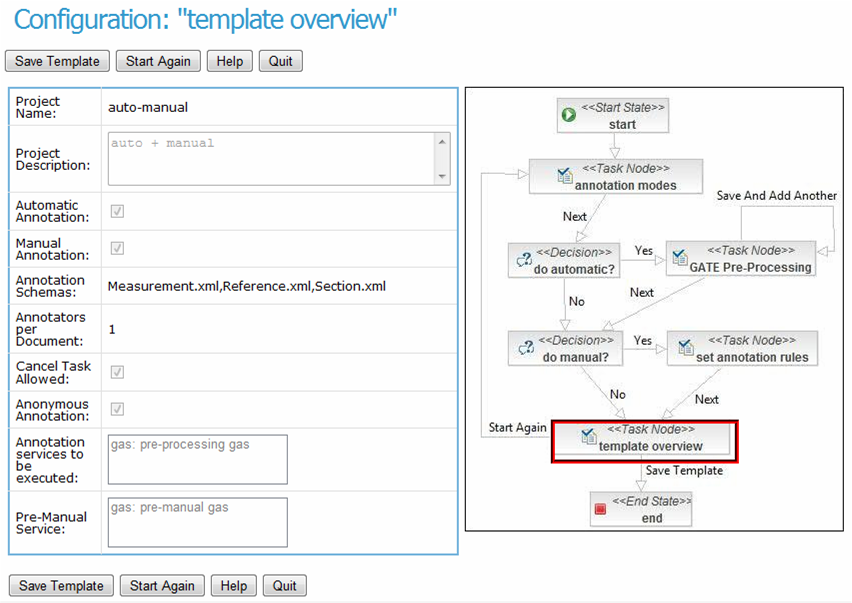
\includegraphics[scale=0.7]{treamware-workflow-example.png}
\caption{Dynamic Workflow Configuration: Example} \label{fig:workflowExample}
\end{center}
\end{figure*}

\subsection{Annotation Services}

The Annotation Services (GAS) provide distribution of compute-intensive NLP tasks over multiple processors. It is transparent to the external user how many machines are actually used to execute a particular service. GAS provides a straightforward mechanism for running applications, created with the GATE framework, as web services that carry out various NLP tasks. In practical applications we have tested a wide range of services such as named entity recognition (based on the freely-available ANNIE system \cite{Cun02b}), ontology population \cite{Maynard09b}, patent processing \cite{Agatonovic08}, and automatic adjudication of multiple annotation layers in corpora. 

The GAS architecture is itself layered, with a separation between the web service endpoint that accepts requests from clients and queues them for processing, and one or more \emph{workers} that take the queued requests and process them.  The queueing mechanism used to communicate between the two sides is the Java Messaging System (JMS)\footnote{http://java.sun.com/products/jms/}, a standard framework for reliable messaging between Java components, and the configuration and wiring together of all the components is handled using the Spring Framework \footnote{http://www.springsource.org/}.

The endpoint, message queue and worker(s) are conceptually and logically separate, and may be physically hosted within the same Java Virtual Machine (VM), within separate VMs on the same physical host, or on separate hosts connected over a network.  When a service is first deployed it will typically be as a single worker which resides in the same VM as the service endpoint.  This may be adequate for simple or lightly-loaded services but for more heavily-loaded services additional workers may be added dynamically without shutting down the web service, and similarly workers may be removed when no longer required.  All workers that are configured to consume jobs from the same endpoint will transparently share the load.  Multiple workers also provide fault-tolerance -- if a worker fails its in-progress jobs will be returned to the queue and will be picked up and handled by other workers.  

\subsection{The Executive Layer}\label{sect:executive}

Firstly, the executive layer implements authentication and user management, including role definition and assignment. In addition, administrators can define here which UI components are made accessible to which user roles (the defaults are shown in Figure~\ref{fig:architecture}). 

The second major part is the workflow manager, which is based on JBoss jBPM\footnote{http://www.jboss.com/products/jbpm/} and has been developed to meet most of the requirements discussed in Section~\ref{sect:workflow-reqs} above. Firstly, it provides dynamic workflow management: create, read, update, delete (CRUD) workflow definitions, and workflow actions. Secondly, it supports business process monitoring, i.e., measures how long annotators take, how good they are at annotating, as well as reporting the overall progress and costs. Thirdly, there is a workflow execution engine which runs the actual annotation projects. As part of the execution process, the project manager selects the number of annotators per document; the annotation schemas; the set of annotators and curator(s) involved in the project; and the corpus to be annotated. 

Figure~\ref{fig:workflowExample} shows an example workflow template. The diagram on the right shows the choice points in workflow templates - whether to do automatic annotation or manual or both; which automatic annotation services to execute and in what sequence; and for manual annotation -- what schemas to use, how may annotators per document, whether they can reject annotating a document, etc. The left-hand side shows the actual selections made for this particular workflow, i.e., use both automatic and manual annotation; annotate measurements, references, and sections; and have one annotator per document. Once this template is saved by the project manager, then it can be executed by the workflow engine on a chosen corpus and list of annotators and curators. The workflow engine will first call the automatic annotation service to bootstrap and then its results will be corrected by human annotators. 

\begin{figure*}[t!]
\begin{center}
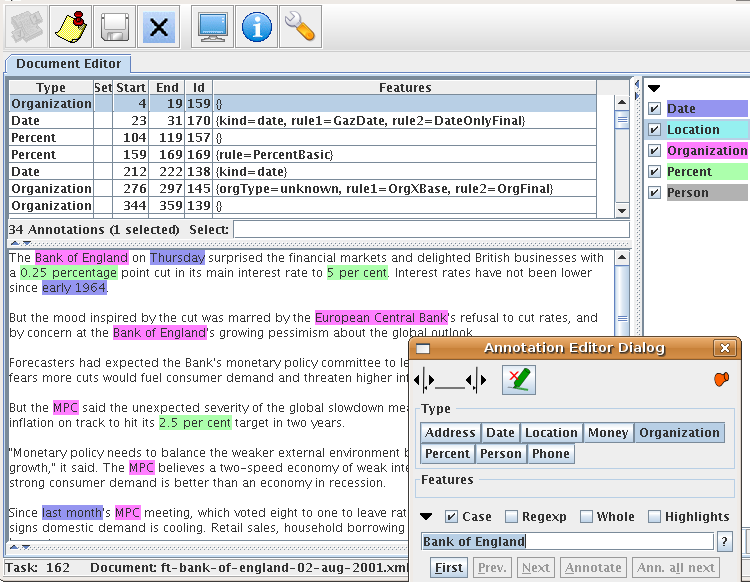
\includegraphics[scale=0.5]{teamware-ann-gui-annon.png}
\caption{The Schema-based Annotator UI} \label{fig:annGUI}
\end{center}
\end{figure*}

The rationale behind having an executive layer rather than defining authentication 
and workflow management as services similar to the storage and ontology ones 
comes from the fact that Teamware services are all SOAP web services, whereas
elements of the executive layer are only in part implemented as SOAP services with the
rest being browser based. Conceptually also the workflow manager acts like a middleman that ties 
together all the different services and communicates with the user interfaces.

\subsection{The User Interfaces}

The \teamware\ user interfaces are web-based and do not require prior installation. They either rendered natively in the web browser or, for more complex UIs, a Java Web Start wrapper is provided around some Swing-based GATE editors (e.g., the document editor and the ANNIC viewer \cite{Aswani05}). After the user logs in, the system checks their role(s) and access privileges to determine which interface elements they are allowed to access. 

\subsubsection{Annotator User Interface}

When manual annotators log into \teamware, they see a very simple web page with one link to their user profile data and another one -- to start annotating documents. The generic schema-based annotator UI is shown in Figure~\ref{fig:annGUI} and it is a visual component in GATE, which is reused here via Java Web Start\footnote{http://java.sun.com/javase/technologies/desktop/javawebstart/index.jsp}. This removes the need to install GATE on the annotator machines and instead they just click on a link to download and start a web application. 

The annotation editor dialog shows the annotation types (or tags) valid for the current project and optionally their features (or attributes). These are generated automatically from the annotation schemas assigned to the project by its manager. The annotation editor also supports the modification of annotation boundaries, as well as the use of regular expressions to annotate multiple matching strings simultaneously. To add a new annotation, one selects the text with the mouse (e.g., ``Bank of England'') and then clicks on the desired annotation type in the dialog (e.g., Organization). Existing annotations are edited by hovering over them, which shows their current type and features in the editor dialog. 

The toolbar at the top of Figure~\ref{fig:annGUI} shows all other actions which can be performed. The first button requests a new document to be annotated. When pressed, a request is sent to the workflow manager which checks if there are any pending documents which can be assigned to this annotator. The second button signals task completion, which saves the annotated document as completed on the data storage layer and enables the annotator to ask for a new one (via the first button). The third (save) button stores the document without marking it as completed in the workflow. This can be used for saving intermediary annotation results or if an annotator needs to log off prior to completing a document. The next time they login and request a new task, they will be given this document to complete first.   

\subsubsection{Curator User Interface}

As discussed above, curators (or editors) carry out quality assurance tasks. In \teamware\ the curation tools cover IAA metrics (e.g. precision/recall and kappa) to identify if there are differences between annotators; a visual annotation comparison tool to see quickly where the differences are per annotation type \cite{Cun02b}; and an editor to edit and reconcile annotations manually (i.e., adjudication) or by using external automatic services. 

\begin{figure*}[t!]
\begin{center}
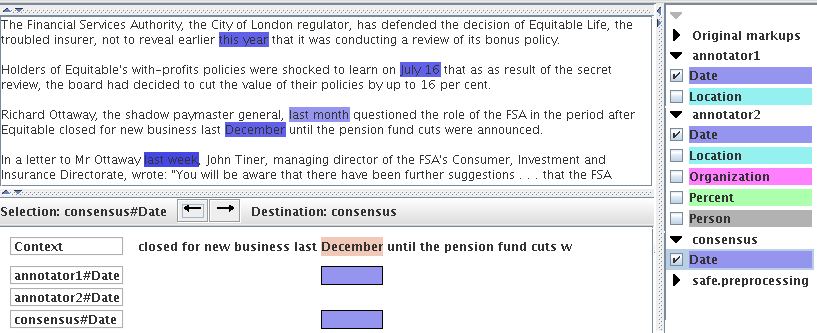
\includegraphics[scale=0.6]{teamware-curator-adjudication.png}
\caption{Part of the Adjudication UI} \label{fig:curatorGUI}
\end{center}
\end{figure*}

The key part of the manual adjudication UI is shown in Figure~\ref{fig:curatorGUI}: the complete UI shows also the full document text above the adjudication panel, as well as lists all annotation types on the right, so the curator can select which one they want to work on. In our example, the curator has chosen to adjudicate Date annotations created by two annotators and to store the results in a new consensus annotation set. The adjudication panel has on top arrows that allow curators to jump from one difference to the next, thus reducing the required effort. The relevant text snippet is shown and below it are shown the annotations of the two annotators. The curator can easily see the differences and correct them, e.g., by dragging the correct annotation into the consensus set.  

\subsubsection{Project Manager Interface}

The project manager web UI is the most powerful and multi-functional one. It provides the front-end to the executive layer (see Section~\ref{sect:executive} and Figure~\ref{fig:workflowExample}). In a nutshell, managers upload documents and corpora, define the annotation schemas, choose and configure the workflows and execute them on a chosen corpus. The management console also provides project monitoring facilities, e.g., number of annotated documents, number in progress, and yet to be completed (see Figure~\ref{fig:monitorGUI}). Per annotator statistics are also available -- time spent per document, overall time worked, average IAA, etc. These requirements were discussed in further detail in Section~\ref{sect:multi-role-support} above.

\begin{figure}[h!]
\begin{center}
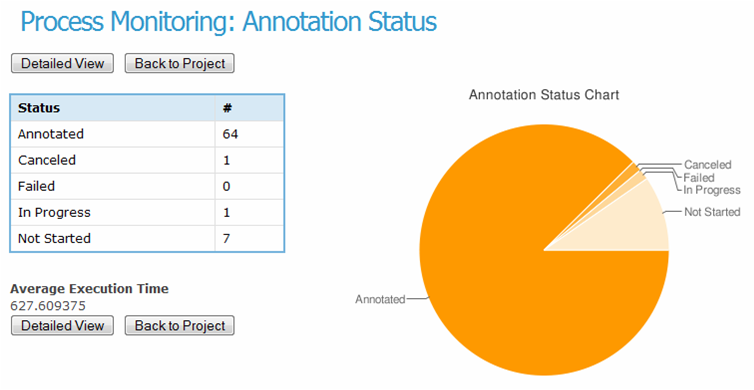
\includegraphics[scale=0.35]{teamware-project-stats.png}
%\vspace{-4.0ex}
\caption{Project Progress Monitoring UI} \label{fig:monitorGUI}
\end{center}
\end{figure}
%\vspace{-6.0ex}

\section{Practical Applications}\label{sect:applications}

\teamware\ has already been used in practice in over 10 corpus annotation projects of varying complexity and size -- due to space limitations, here we focus on three representative ones. Firstly, we tested the robustness of the data layer and the workflow manager in the face of simultaneous concurrent access. For this we annotated 100 documents, 2 annotators per document, with 60 active annotators requesting documents to annotate and saving their results on the server. There were no latency or concurrency issues reported. 

Once the current version was considered stable, we ran several corpus annotation projects to produce gold standards for IE evaluation in three domains: business intelligence, fisheries, and bio-informatics. The latter involved 10 bio-informatics students which were first given a brief training session and were then allowed to work from home. The project had 2 annotators per document, working with 6 entity types and their features. Overall, 109 Medline abstracts of around 200-300 words each were annotated with average annotation speed of 9 minutes per abstract. This project revealed several shortcomings of \teamware\ which will be addressed in the forthcoming version 2: 
\begin{itemize}
  \item  IAA is calculated per document, but there is no easy way to see how it changes across the entire corpus. 
  \item The datastore layer can sometimes leave the data in an inconsistent state following an error, due to the underlying binary Java serialisation format. A move towards XML file-based storage is being investigated.
  \item There needs to be a limit on the proportion of documents which any given annotator is allowed to work on, since one over-zealous annotator ended up introducing a significant bias by annotating more than 80\% of all documents. 
\end{itemize}    

The most versatile and still ongoing practical use of \teamware\ has been in a commercial context, where a company has two teams of 5 annotators each (one in China and one in the Philippines). The annotation projects are being defined and overseen by managers in the USA, who also act occasionally as curators. They have found that the standard double-annotated agreement-based approach is a good foundation for their commercial needs (e.g., in the early stages of the project and continuously for gold standard production), while they also use very simple workflows where the results of automatic services are being corrected by annotators, working only one per document to maximise volume and lower the costs. In the past few months they have annotated over 1,400 documents, many of which according to multiple schemas and annotation guidelines. For instance, 400 patent documents were doubly annotated both with measurements (IAA achieved 80-95\%) and bio-informatics entities, and then curated and adjudicated to create a gold standard. They also annotated 1000 Medline abstracts with species information where they measured average speed of 5-7 minutes per document. The initial annotator training in Teamware was between 30 minutes and one hour, following which they ran several small-scale experimental projects to train the annotators in the particular annotation guidelines (e.g., measurements in patents). Annotation speed also improved over time, as the annotators became more proficient with the guidelines -- the Teamware annotator statistics registered improvements of between 15 and 20\%. Annotation quality (measured through inter-annotator agreement) remained high, even when annotators have worked on many documents over time. 

